\chapter{Event Reconstruction and Selection}

\section{Physics Objects}
\label{section:objects}
The physics objects in this thesis are reconstructed using a modified particle flow (PF) algorithm for the \textsc{Delphes} parametrization of the detector geometry. The PF algorithm combines information from the tracker, the calorimeters, and the muon system to form PF candidates~\cite{cms:pf2017}.

The most crucial element of this thesis is identifying the Higgs boson decaying to two b quarks. Because quarks cannot exist independently, the b quarks will quickly hadronize. These hadrons show up in the detector through the tracks they make in the silicon tracker and the energy they deposit in the HCAL. The anti-$k_T$ clustering algorithm~\cite{ak2008} then combines the PF candidates from those tracks and HCAL hits to form jets. In particular, it forms AK4 and AK8 jets (so-called because they are clustered within radii of $R=0.4$ and $R=0.8$, respectively). As can be seen in \cref{fig:deltaRvspt}, b quarks from the decays of a high-momentum Higgs boson are more likely than not to be within $R=0.8$ from each other. As a result, AK8 jets that are reconstructed from the decays of such Higgs bosons will typically contain both b quarks in the jet radius. Accordingly, they are a key focus of this search since the signal will almost certainly be reconstructed as an AK8 jet. The extreme PU of the Phase-2 detector, described earlier, is accounted for with the Pileup Per Particle Identification (PUPPI) algorithm~\cite{puppi2014}.

Because of the limited extent of the tracker, AK4 and AK8 jets must be within $|\eta|$ of $3.0$. AK8 jets must have a \pt of at least $\GeV{200}$, while AK4 jets must have a \pt of at least $\GeV{30}$ . Both jets need to pass basic identification requirements~\cite{CMS-DP-2020-020} and are additionally removed if a lepton is contained within their radius, so as to prevent double-counting of jets that are also identified as leptons. The AK8 jet mass is calculated with the soft drop (SD) algorithm~\cite{sd2014}. It is important to note that, although AK4 jets and AK8 jets can be reconstructed from the same PF candidates, AK4 jets that are found within the AK8 jet cone are not removed. As a result, overlap between these objects is possible.

\begin{figure}[ht]
\centering
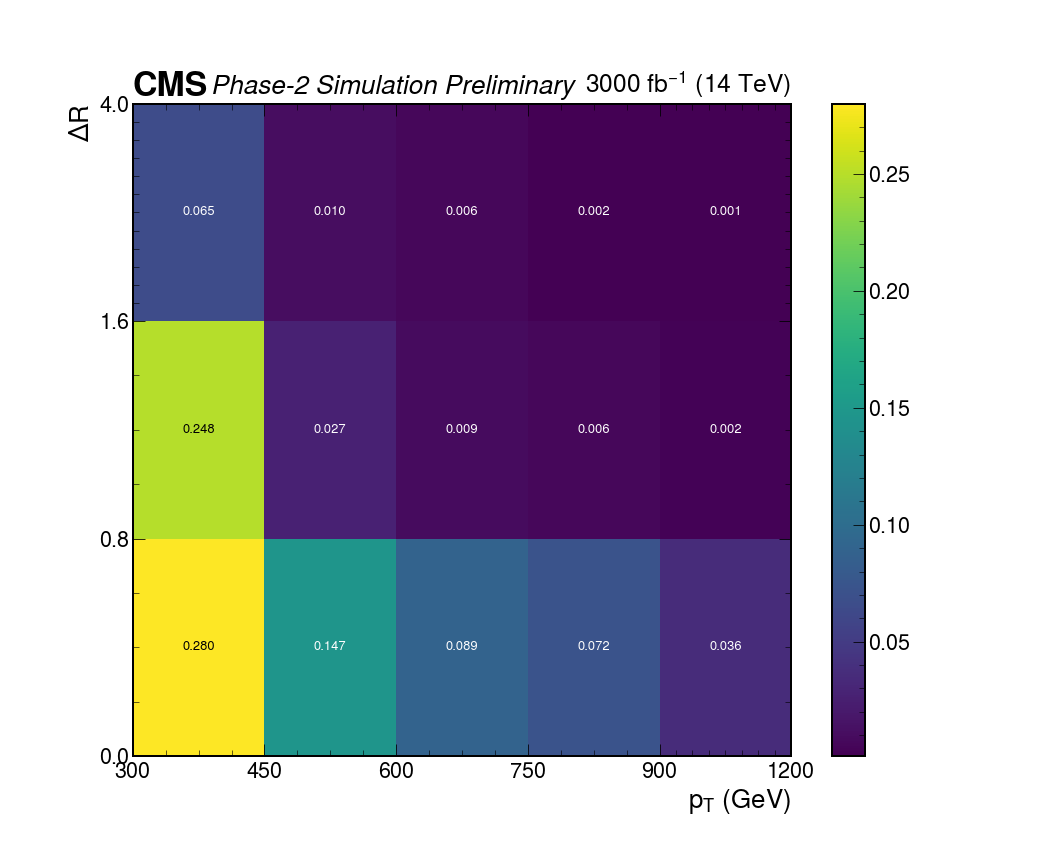
\includegraphics[width=0.845\textwidth]{Chapters/Strategy/b_DeltaR_vs_h_pt.png}
\caption{The $\Delta R$ between two generator-level b quarks against the \pt of the generator-level Higgs boson in events from a 2HDM+a signal with $m_\mathrm{A} = 1900$ GeV, $m_\mathrm{a} = 250$ GeV. The value in each bin in this histogram is the ratio of the counts in that bin to the overall yield.}
\label{fig:deltaRvspt}
\end{figure}

The \ptvecmiss is calculated using the vector sum of the \pt of the PF candidates, with inputs from the PUPPI algorithm to mitigate the effects of PU.

One tool often used in analyses that focus on particles such as the Higgs boson are heavy object taggers. These are algorithms created using machine learning techniques that excel at identifying objects such as the Higgs boson from a variety of similar looking backgrounds. In particular, taggers were developed during Run 2 of the LHC to identify AK8 jets that arise from Higgs decays to b$\bar{\mathrm{b}}$~\cite{CMS:2020mlt, Qu_2020}. Unfortunately, no such taggers are implementable for the \textsc{Delphes} framework. However, I anticipate that the accuracy of such taggers is likely to be at least as performant during the HL-LHC era.

Using fully simulated LHC Run 2 samples, the tagger efficiency is parametrized as a function of the AK8 jet \pt and $|\eta|$. The true efficiency of the tagger, when the tagger accurately identifies a Higgs boson, is calculated for events with generator-level Higgs bosons contained in the AK8 jet cone. The mistag efficiency, when the tagger mistakenly identifies a Higgs boson, is further parametrized by the number of b quarks in the AK8 jet cone. The efficiency is calculated by binning the simulated events in these variables, then calculating the efficiency in each bin according to \cref{eq:tageff}. A jet is considered tagged if it passes a working point based on the performance of the DeepAK8Jet mass-decorrelated h $\to$ b$\bar{\mathrm{b}}$ tagger against a multijet background. The efficiency is calculated on a sample-by-sample basis, owing to the sample-dependent nature of the tagger. A qualitative example of the mistag efficiencies for events with zero, one, or two b quarks in a semileptonic t$\bar{\mathrm{t}}$ sample is shown in \cref{fig:tagger}. After the tagger efficiency is calculated, it is then applied as a weight to the \textsc{Delphes} events as a function of the parametrized variables. The efficiency is calculated for each AK8 jet in the event as a function of \pt, $|\eta|$, and the number of b quarks and Higgs bosons in the AK8 jet cone. The weights for events with either no Higgs bosons or one or more Higgs bosons are then calculated according to the formulas given in \cref{eq:w0h,eq:w1h}.

\begin{equation}
    \epsilon = \frac{N_\text{tagged}}{N_\text{jets}}
    \label{eq:tageff}
\end{equation}

\begin{figure}[ht]
\centering
\begin{subfigure}[b]{0.33\textwidth}
         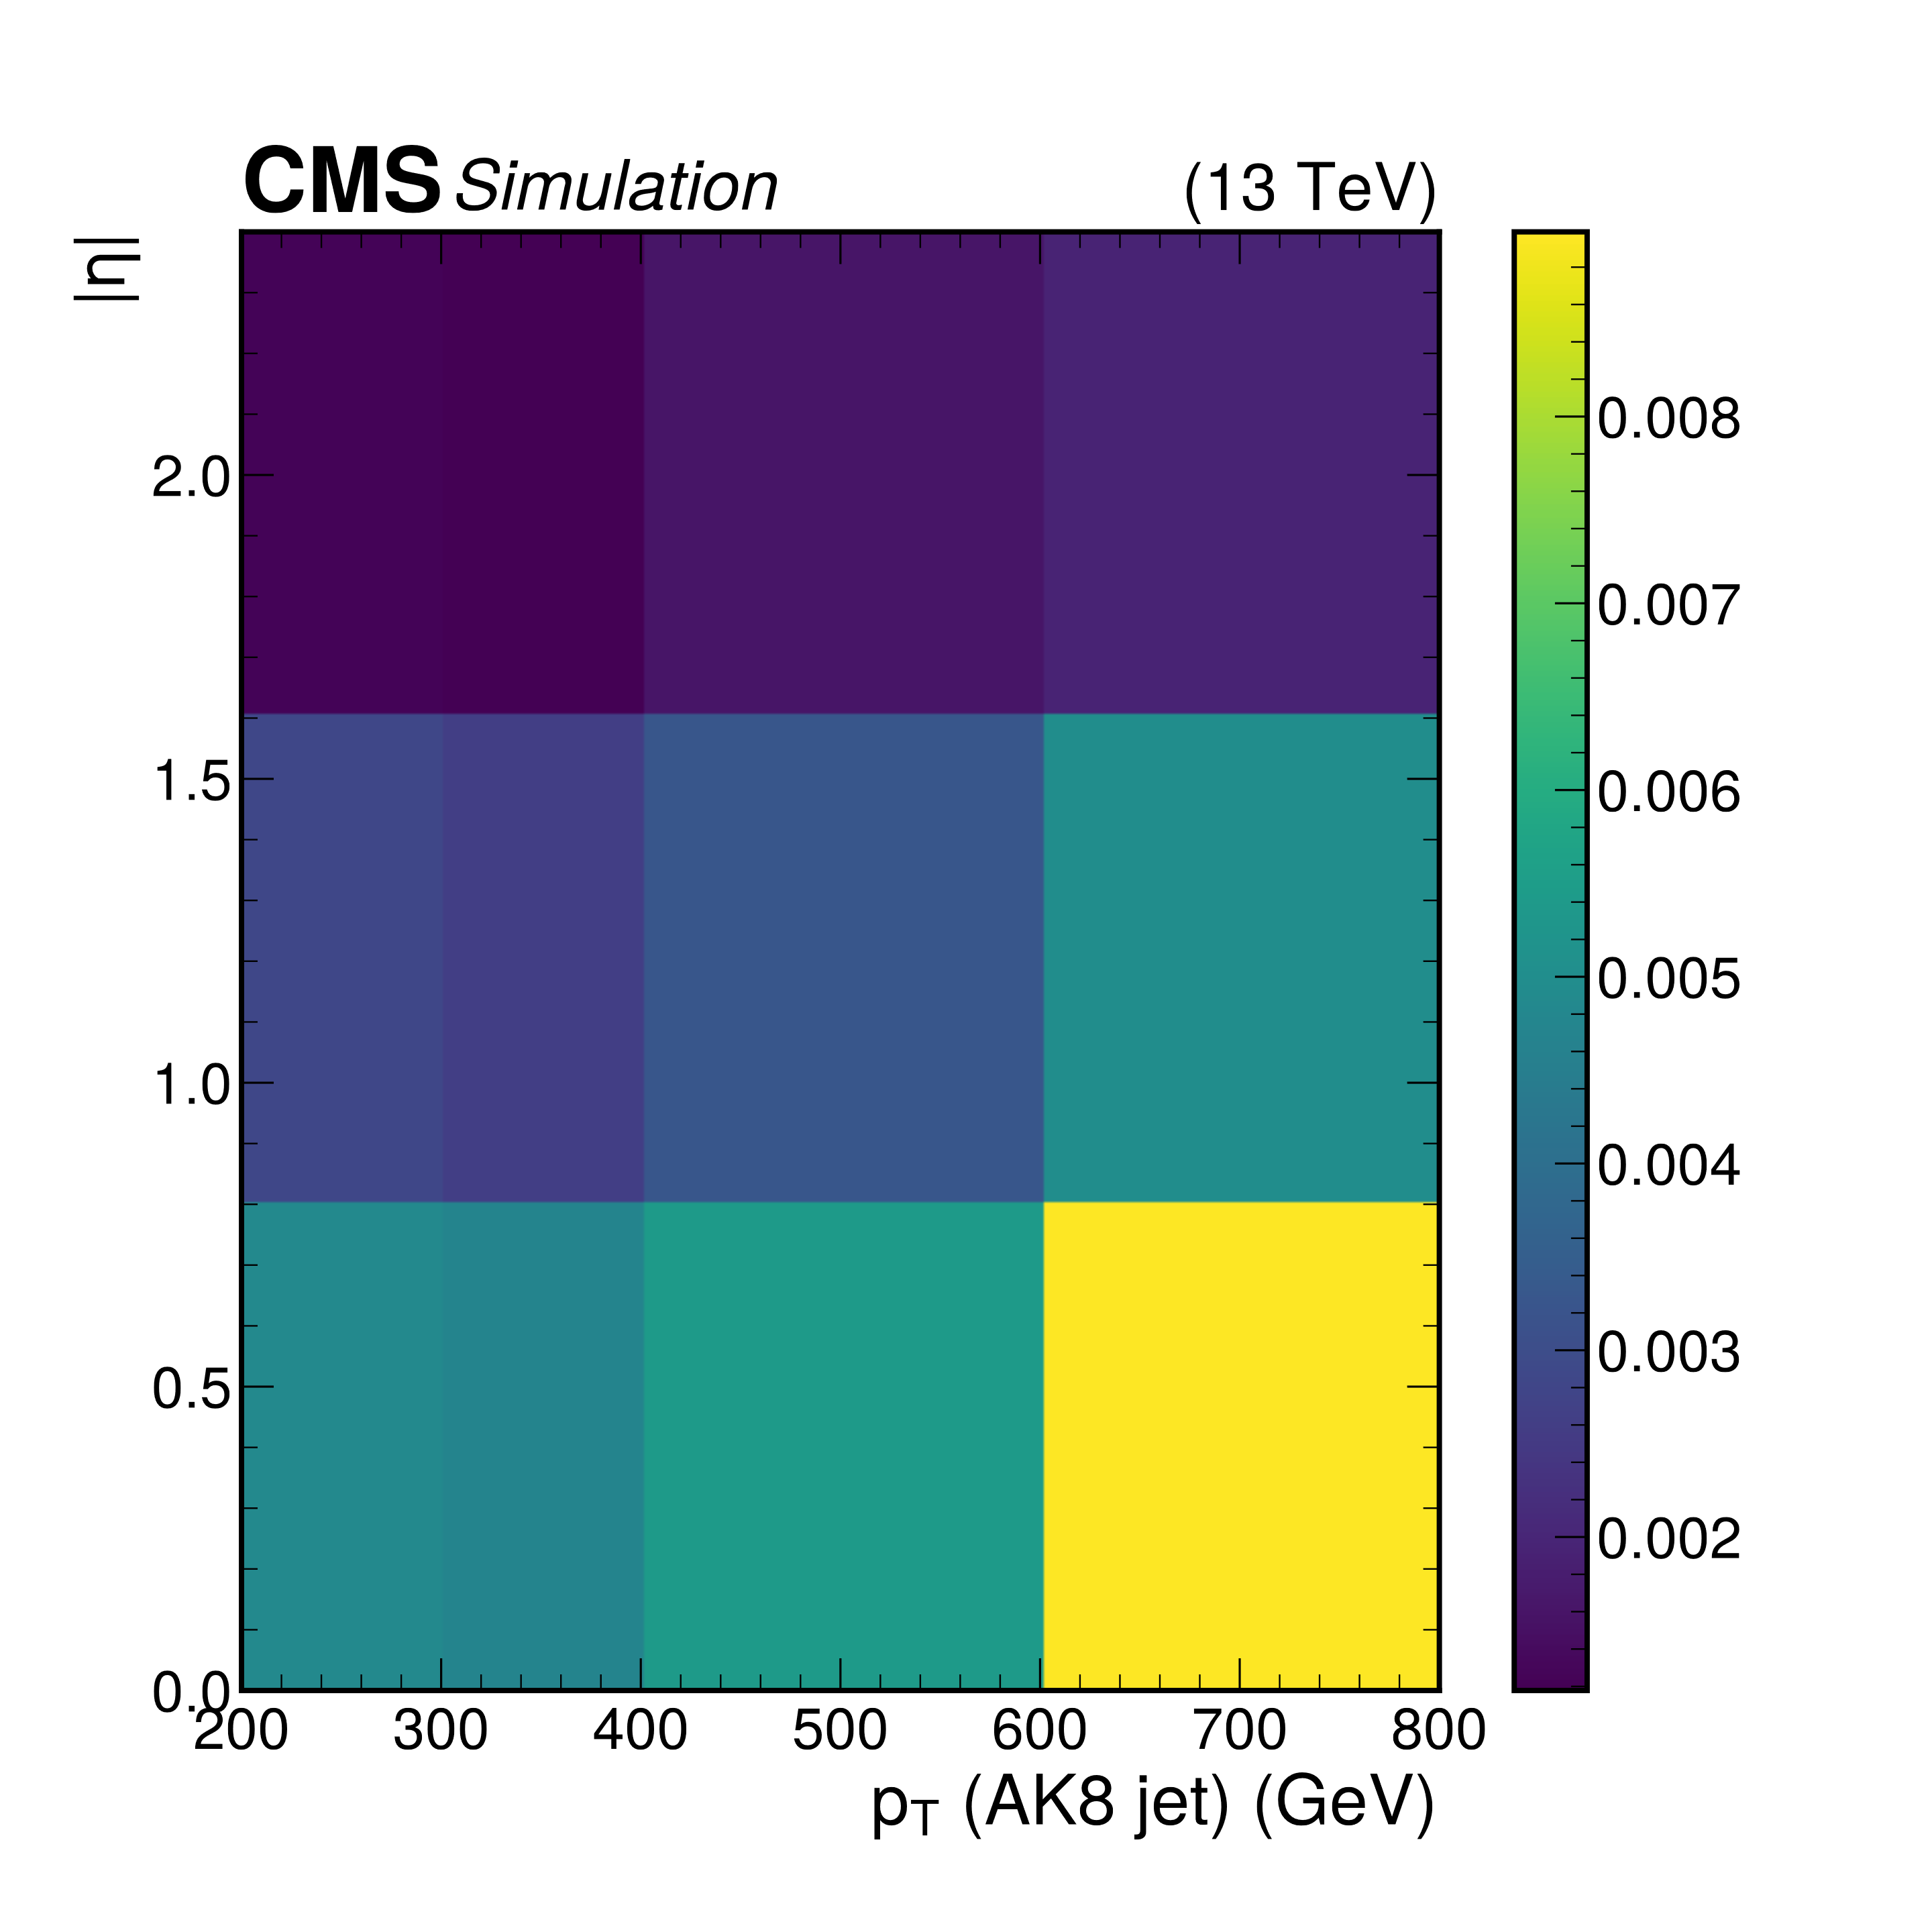
\includegraphics[width=\textwidth]{Chapters/Strategy/0b.png}
         \caption{The mistag efficiencies for zero b quarks.}
     \end{subfigure}
     \begin{subfigure}[b]{0.33\textwidth}
         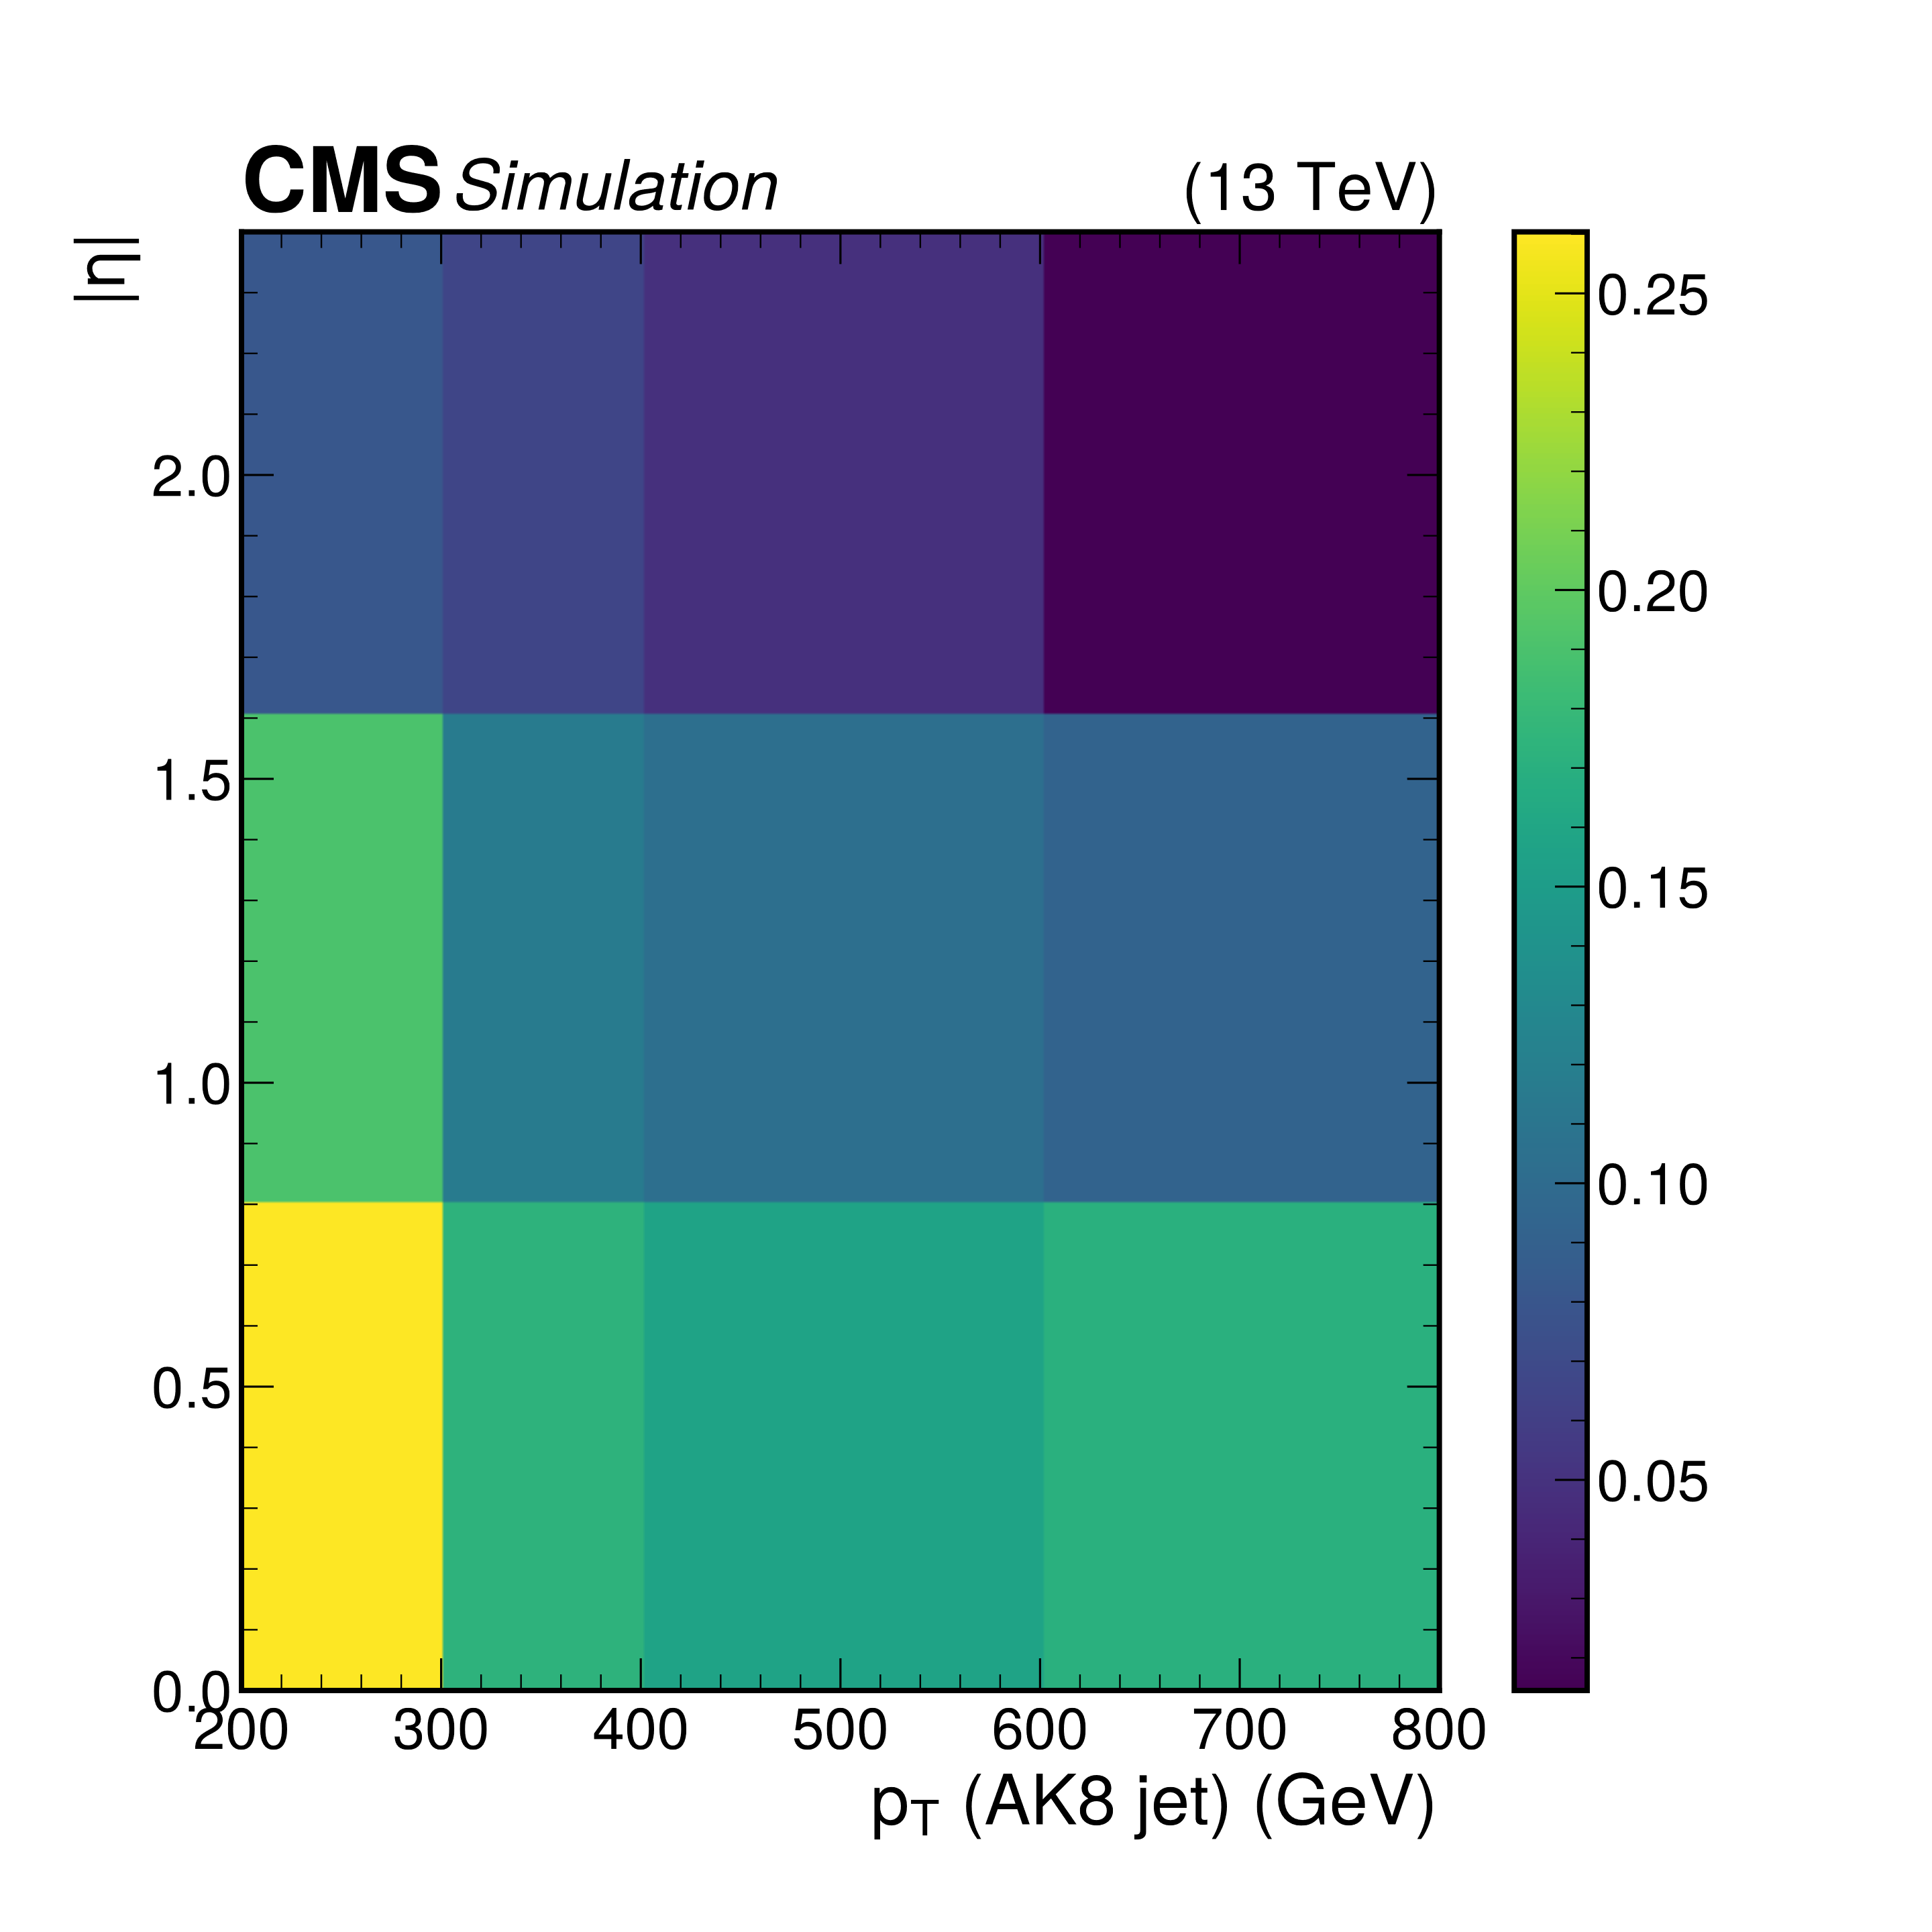
\includegraphics[width=\textwidth]{Chapters/Strategy/1b.png}
         \caption{The mistag efficiencies for one b quark.}
     \end{subfigure}
    \begin{subfigure}[b]{0.33\textwidth}
         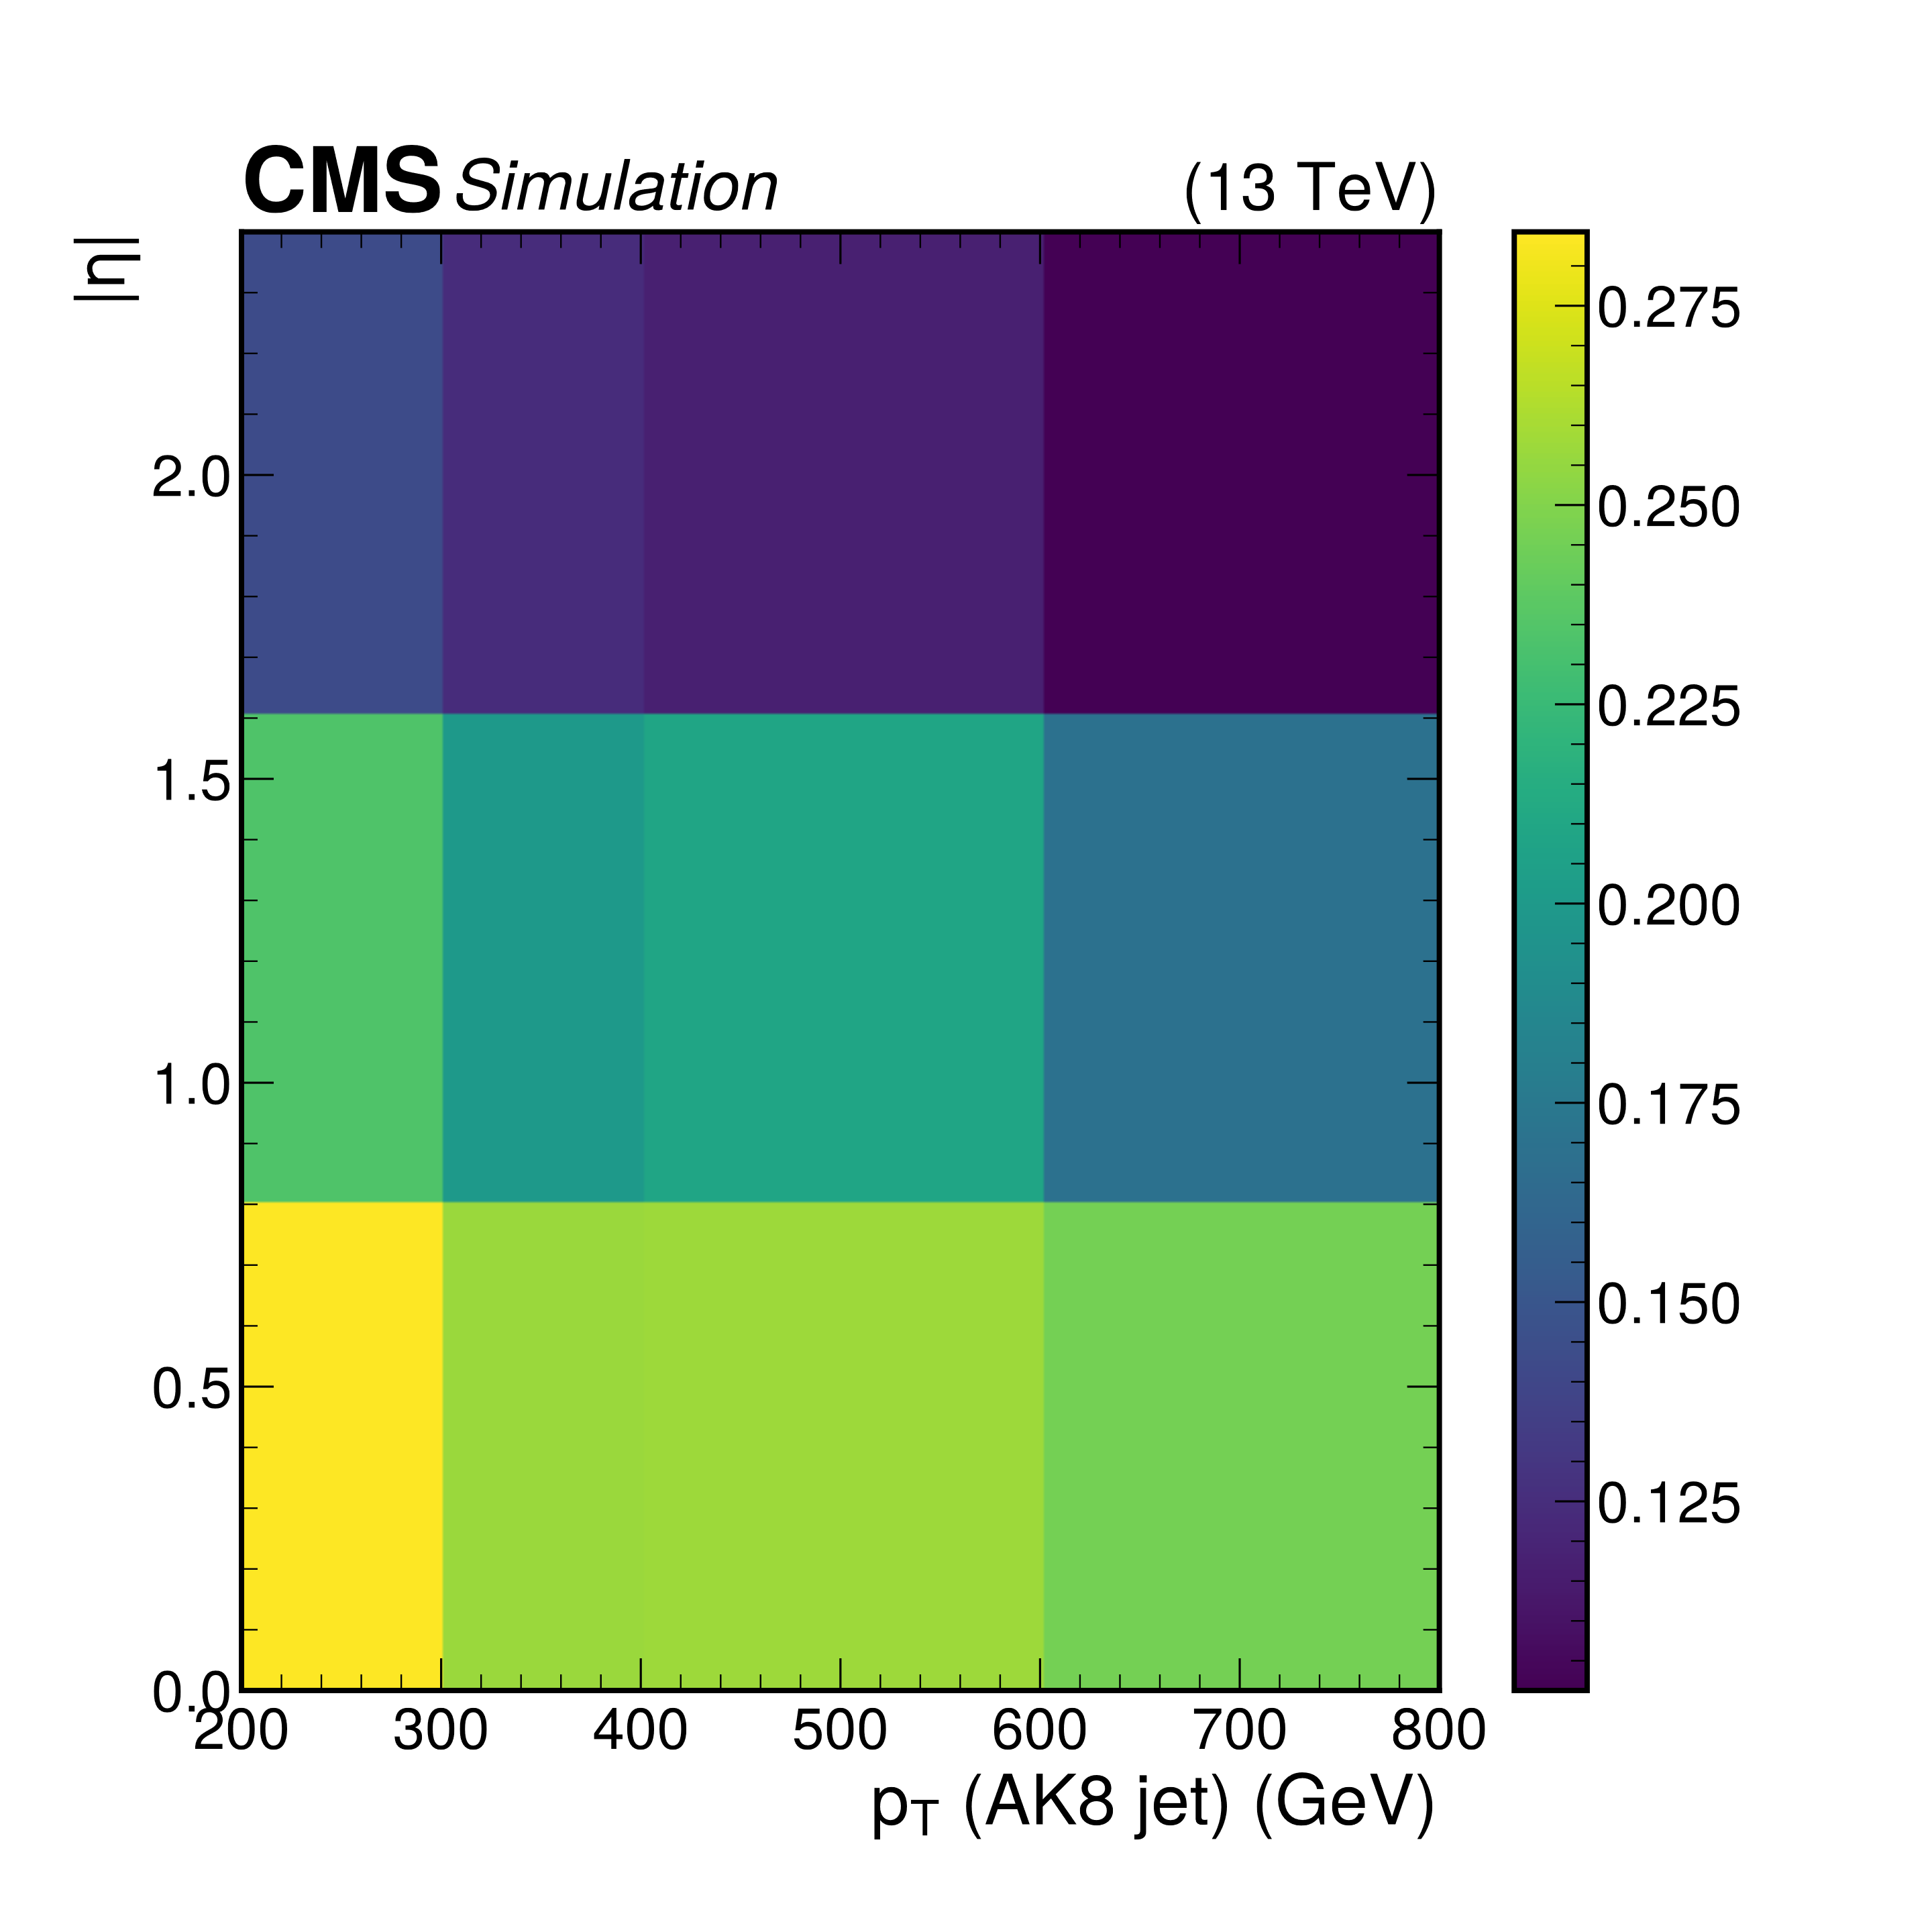
\includegraphics[width=\textwidth]{Chapters/Strategy/2b.png}
         \caption{The mistag efficiencies for two b quarks.}
     \end{subfigure}
\caption{\raggedright The mistag efficiencies of the Run 2 h $\to$ b$\bar{\mathrm{b}}$ mass-decorrelated DeepAK8Jet tagger in a semileptonic t$\bar{\mathrm{t}}$ sample. The efficiency has been parametrized as a function of \pt and $|\eta|$.}
\label{fig:tagger}
\end{figure}

\begin{equation}
    w(\text{0h}) = \prod_{i\in\text{\{AK8 jets\}}}(1-\epsilon_i)
    \label{eq:w0h}
\end{equation}

\begin{equation}
    w(\geq\text{1h}) = 1 - w(\text{0h})
    \label{eq:w1h}
\end{equation}

Leptons in the detector are reconstructed from their tracks and their deposits in the ECAL. Muons are additionally reconstructed using information from the muon system and taus can be reconstructed with deposits in the HCAL. Leptons represent an important part of the thesis because removing lepton final states eliminates a substantial portion of the background in this search. The Phase-2 detector is enormously beneficial in doing so, as it expands the geometric coverage of leptons in the detector. Electrons are required to have a \pt greater than $\GeV{10}$ and have $|\eta| < 3.0$. Muons are required to have a \pt greater than $\GeV{4}$ and have $|\eta| < 2.8$. Taus are required to have a \pt greater than $\GeV{30}$ and have $|\eta| < 3.0$. In addition, the leptons are required to pass identification and isolation restrictions. For electrons and muons, the relative isolation as defined in \cref{eq:irel} is required to be less than 0.3. The identification requirements for electrons and muons in \textsc{Delphes} are based on the identification requirements from the full simulation of the Phase-2 samples. The tau isolation requirements are based on machine learning tools designed to identify taus from jets. A summary of the object selections is given in \cref{tab:objdef}.

\begin{equation}
    \text{Iso}_{\text{rel}} = \frac{\sum \pt(\text{PUPPI particles within } R=0.3)}{\pt(\mathrm{e}, \upmu)}
    \label{eq:irel}
\end{equation}

\begin{table}[ht!]
  \centering
  \caption{Object selections as described in \cref{section:objects}}
  \begin{tabular}{|c|c|c|c|c|}
    \hline
    Object & \pt (GeV) $>$ & $|\eta|$ $<$ & Iso & ID WP \\
    \hline
    AK4 jet  & 30  & 3.0 &   & L \\
    AK8 jet  & 200 & 3.0 &   & L \\
    electron & 10  & 3.0 & L & L \\
    muon     & 4   & 2.8 & L & L \\
    tau      & 30  & 3.0 & L &   \\
        \hline
    \end{tabular}
    \label{tab:objdef}
\end{table}

 
\section{Event Selection}
Once objects in the detector have been reconstructed, the next step in the search is to remove as many events as possible that could contribute to the background of the signal region. The first few selections are aimed at targeting the final state of a Higgs boson decaying to b$\bar{\mathrm{b}}$ with high \ptmiss. First, the \ptmiss of each event is required to be greater than $\GeV{300}$. This requirement helps ensure that the events in the signal region are in the parameter space the search targets. Additionally, a Phase-2 analysis of this final state would need to use a high \ptmiss threshold in the HLT. As mentioned in the preceding section, one selection is to require that events have no leptons in them. Certain background events such as Z bosons produced in association with initial state jets or other modes of Higgs production can have final states with leptons, so this cut helps to remove much of the initial background. Events are required to have at least one AK8 jet, since signal events should have an AK8 jet from the Higgs decaying to b$\bar{\mathrm{b}}$. At least one AK8 jet in the event should have \pt greater than $\GeV{300}$. Events are also required to have at least 2 AK4 jets. This requirement helps to remove some of the multijet background. Finally, events are required to contain at least one Higgs-tagged AK8 jet. The AK8 jets are not tagged directly, but instead the weight for events with 1 or more Higgs bosons described in \cref{eq:w1h} is applied to all events. By comparing the $m_\text{AK8}$ distribution in a Run 2 sample between events that contained a tagged AK8 jet and events that were reweighted, it can be seen that the two are largely equivalent, as shown in \cref{fig:tagcheck}.

\begin{figure}[ht]
\centering
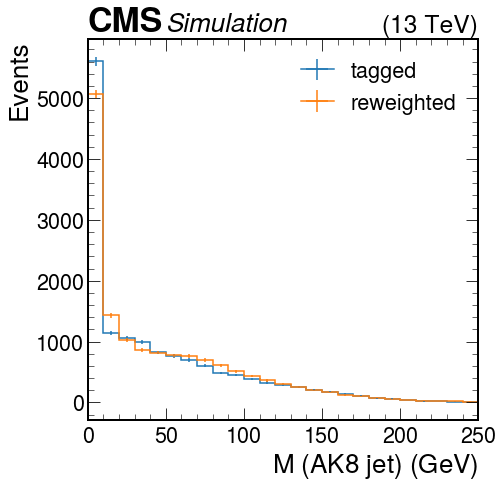
\includegraphics[width=0.6\textwidth]{Chapters/Strategy/tagcheck.png}
\caption{A comparison of the $m_\text{AK8}$ distribution in a Run 2 Z+jets $\to$ $\nu\nu$ sample.}
\label{fig:tagcheck}
\end{figure}

The next set of restrictions on the events is aimed at reducing the prominence of the main backgrounds in the signal region, particularly the multijet background. Jets (either AK8 or AK4) that are closely aligned with the \ptmiss are a sign that the jet momentum is poorly reconstructed in that event, giving rise to the missing momentum. As a result, events are required to have $\Delta\varphi(\text{jets}, \ptvecmiss) > 1$. To further eliminate events with poorly reconstructed jet momenta, events are required to have $\Delta\varphi(\text{AK4 jets}, \ptvecmiss) < 3$. Finally, there is a restriction on jets in a back-to-back configuration, which is a typical sign of multijet production.

As described in \cref{section:2hdma}, under the 2HDM+a model the SM Higgs and the \ptmiss originate from the decay of the pseudoscalar A. $m_\mathrm{A}$ is approximated as

\begin{equation}
    \mt = \sqrt{2\pt(\text{AK8 jets})\ptmiss(1-\cos(\varphi(\text{AK8 jets})-\varphi(\ptvecmiss))}.
    \label{eq:mt}
\end{equation}

This variable is calculated for each AK8 jet, and each event is required to have at least one AK8 jet that has a corresponding \mt of at least $\GeV{600}$.

The baseline event selection is given in \cref{tab:selection}. The relative effectiveness of each selection is shown in \crefrange{fig:metpt}{fig:dphi} where the relevant variable is plotted with each other selection having been applied. Finally, the cumulative effect of the selections is given in \cref{tab:cutflow} which shows the events remaining after each successive selection, split amongst the main background categories and three signals.

\begin{table}
  \centering
  \caption{Summary of the event selection. The requirement that events include at least one h-tagged AK8 means that at least one AK8 jet is required and events are weighted depending on the tagging efficiencies of AK8 jets in the event to mirror the effect of using a Higgs tagger.}
  \begin{tabular}{r|l}
    Observable & Requirement \\
    \hline
    $N_{\text{leptons}}$ & $ = 0$ \\
    \ptmiss & $> \GeV{300}$ \\
    $N_{\text{h-tagged AK8}}$ & $ > 0$ \\
    min $\pt(\text{AK8 jets})$ & $>\GeV{300}$ \\
    $N_{\text{AK4}}$ & $ > 1$ \\
    $\text{min}~ \Delta\varphi(\text{AK8 jets}, \ptvecmiss)$ & $ > 1$ \\
    $\text{min}~ \Delta\varphi(\text{AK4 jets}, \ptvecmiss)$ & 1 -- 3  \\
    $\Delta\varphi(\text{any 2 AK8 jets})$ & $ < 3$ \\
    $\Delta\varphi(\text{any 2 of 4 lead AK4 jets})$ & $ < 3$ \\
    $\text{min}~ \mt(\text{AK8 jets}, \ptvecmiss)$ & $ > \GeV{600}$ \\
  \end{tabular}
  \label{tab:selection}
\end{table}



\begin{figure}[ht]
\centering
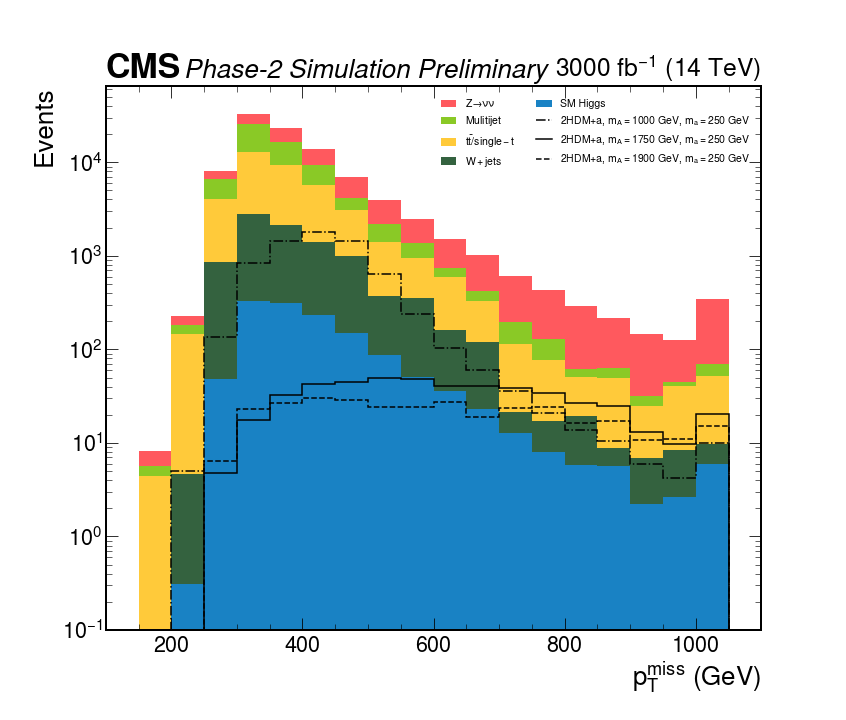
\includegraphics[width=0.845\textwidth]{Chapters/Strategy/selections/met_pt.png}
\caption{The \ptmiss distribution among the backgrounds and the $m_\mathrm{A} =1000$, $1750$, and 
$\GeV{1900}$, $m_\mathrm{a} = \GeV{250}$ signals with each selection except the \ptmiss cut applied.}
\label{fig:metpt}
\end{figure}

\begin{figure}[ht]
\centering
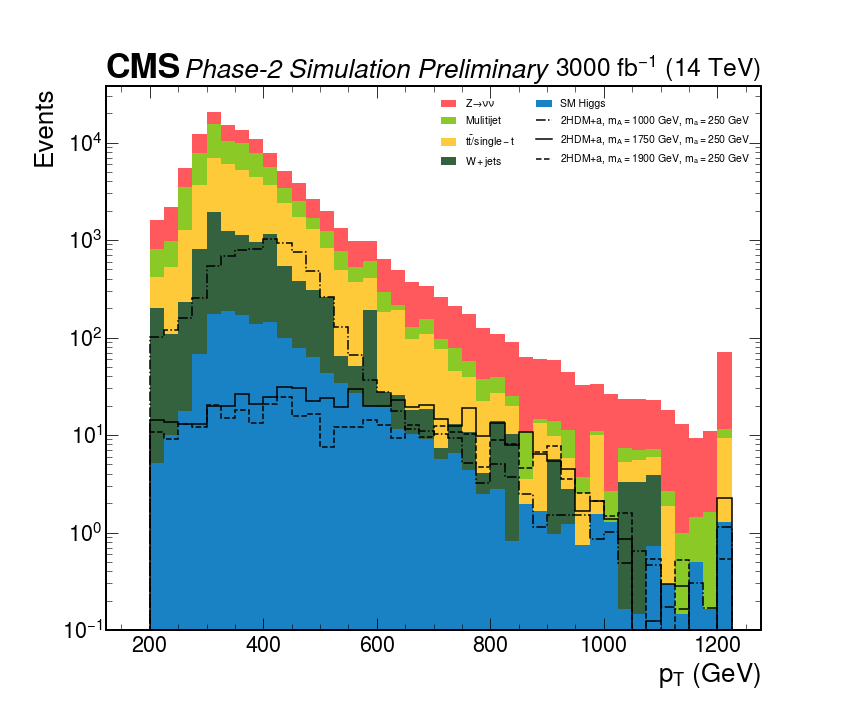
\includegraphics[width=0.845\textwidth]{Chapters/Strategy/selections/min_AK8_pt.png}
\caption{The minimum \pt of the AK8 jets in an event in the backgrounds and the $m_\mathrm{A} =1000$, $1750$, and $\GeV{1900}$, $m_\mathrm{a} = \GeV{250}$ signals with each selection except the min \pt cut applied.}
\label{fig:minak8pt}
\end{figure}

\begin{figure}[ht]
\centering
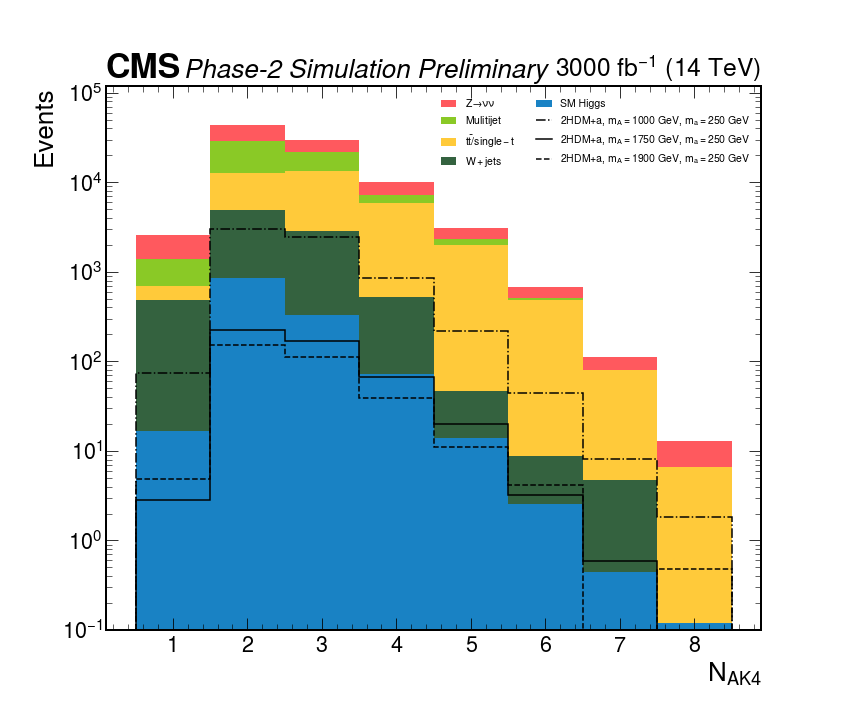
\includegraphics[width=0.845\textwidth]{Chapters/Strategy/selections/n_AK4.png}
\caption{The number of the AK4 jets in each event in the backgrounds and the $m_\mathrm{A} =1000$, $1750$, and $\GeV{1900}$, $m_\mathrm{a} = \GeV{250}$ signals with each selection except the $N_\text{AK4}$ cut applied.}
\label{fig:nak4}
\end{figure}

\begin{figure}[ht]
\centering
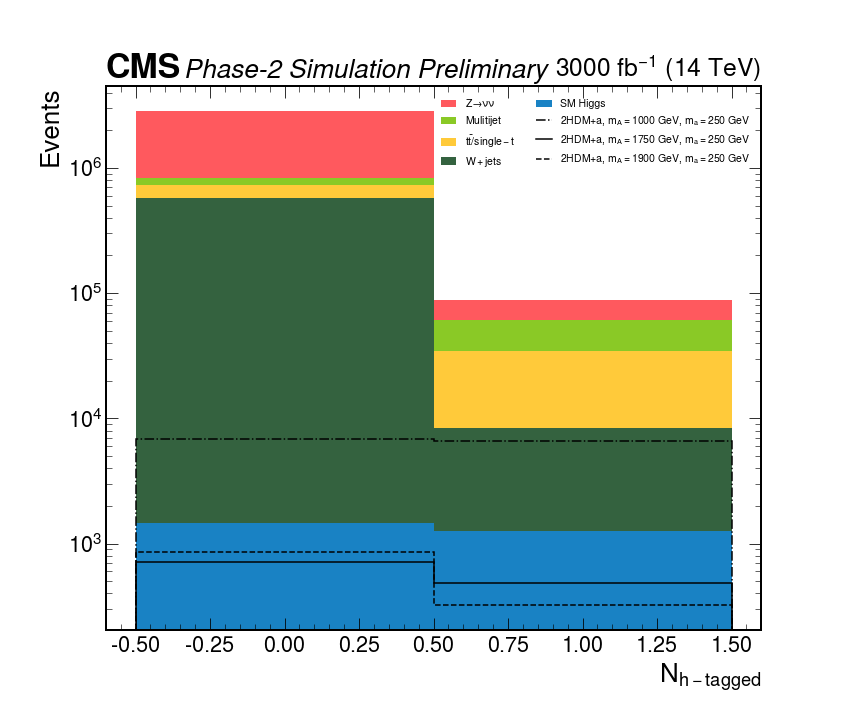
\includegraphics[width=0.845\textwidth]{Chapters/Strategy/selections/NH_weight.png}
\caption{The number of h-tagged jets in the backgrounds and the $m_\mathrm{A} =1000$, $1750$, and $\GeV{1900}$, $m_\mathrm{a} = \GeV{250}$ signals with each selection except the Higgs tagging requirement applied. The Higgs tagging has been done via event weighting, as described above. The right bin is an overflow bin containing all events with one or more h-tagged jets.}
\label{fig:mt}
\end{figure}

\begin{figure}[ht]
    \centering
    
    \begin{subfigure}[b]{0.45\textwidth}
        \centering
        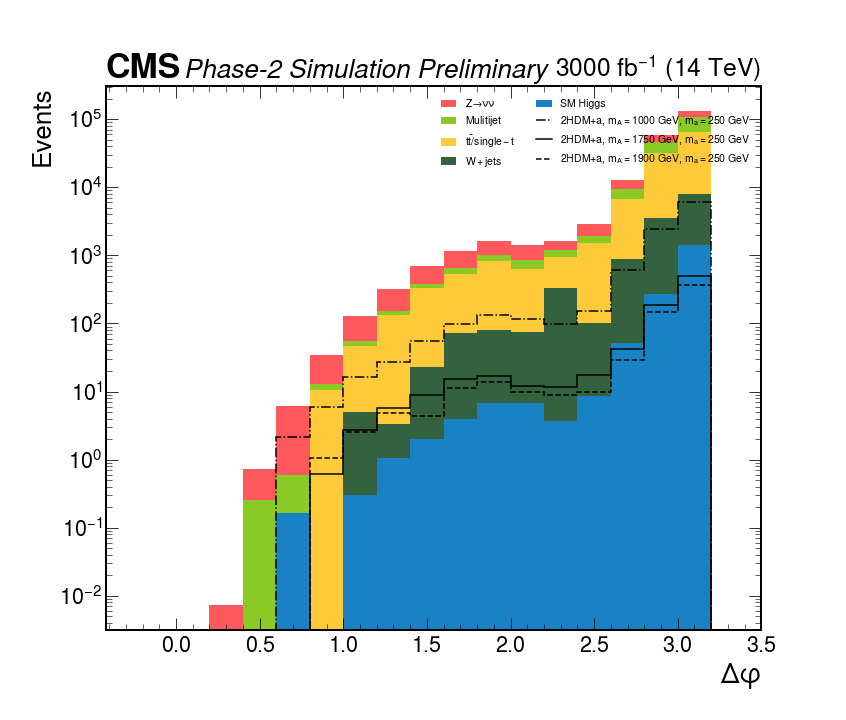
\includegraphics[width=\textwidth]{Chapters/Strategy/selections/dphi_AK8_MET.png}
        \caption{The min $\Delta\varphi(\text{AK8 jets},\ptvecmiss)$ distribution.}
        \label{fig:dphiak8met}
    \end{subfigure}
    \hfill
    \begin{subfigure}[b]{0.45\textwidth}
        \centering
         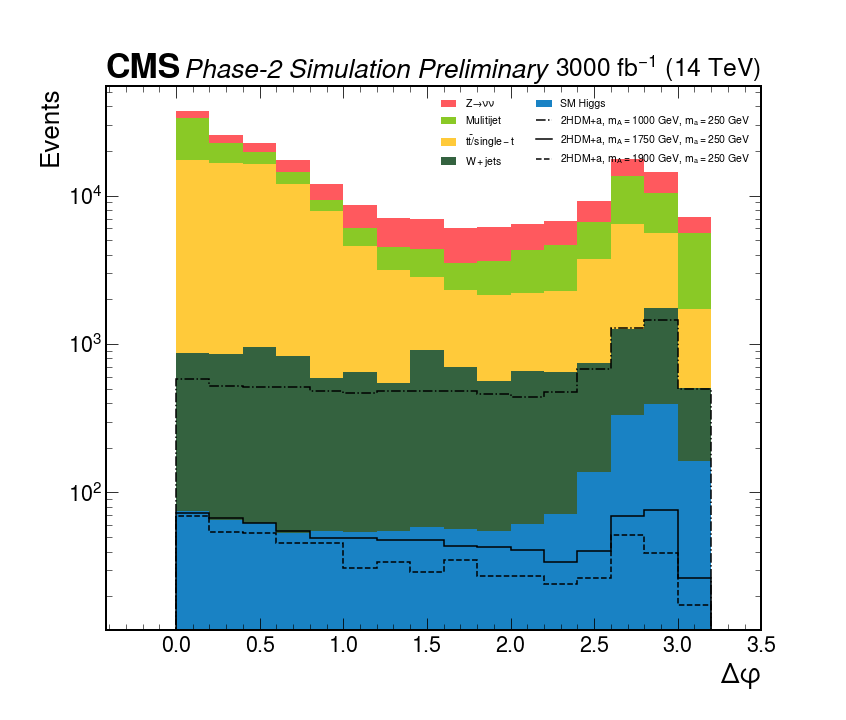
\includegraphics[width=\textwidth]{Chapters/Strategy/selections/dphi_AK4_MET.png}
        \caption{The min $\Delta\varphi(\text{AK4 jets},\ptvecmiss)$ distribution.}
        \label{fig:dphiak4met}
    \end{subfigure}
    
    \begin{subfigure}[b]{0.45\textwidth}
        \centering
        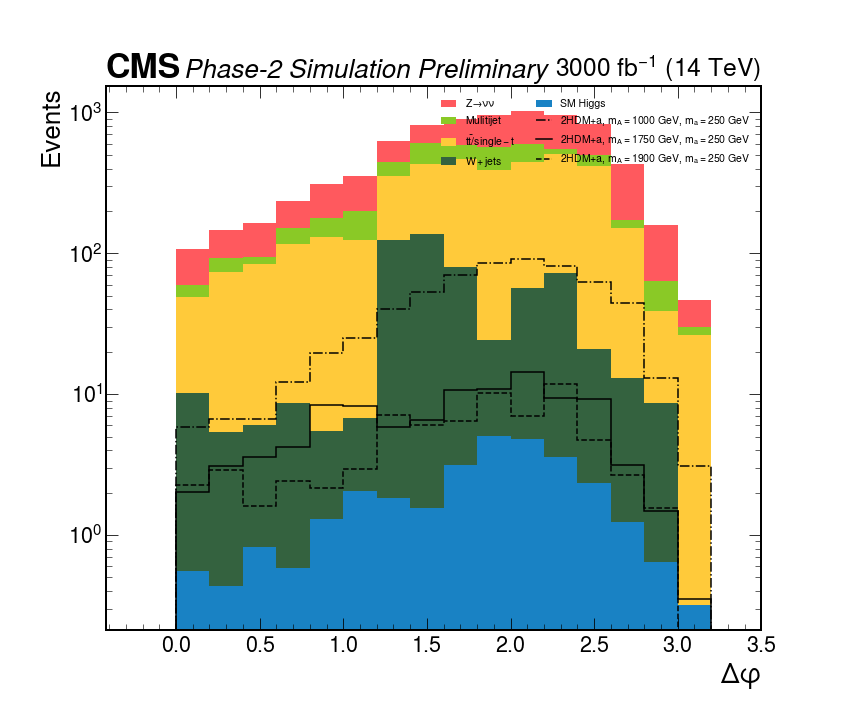
\includegraphics[width=\textwidth]{Chapters/Strategy/selections/AK8_QCD_veto.png}
        \caption{The $\Delta\varphi(\text{any 2 AK8 jets})$ distribution.}
        \label{fig:dphi2ak8}
    \end{subfigure}
    \hfill
    \begin{subfigure}[b]{0.45\textwidth}
        \centering
        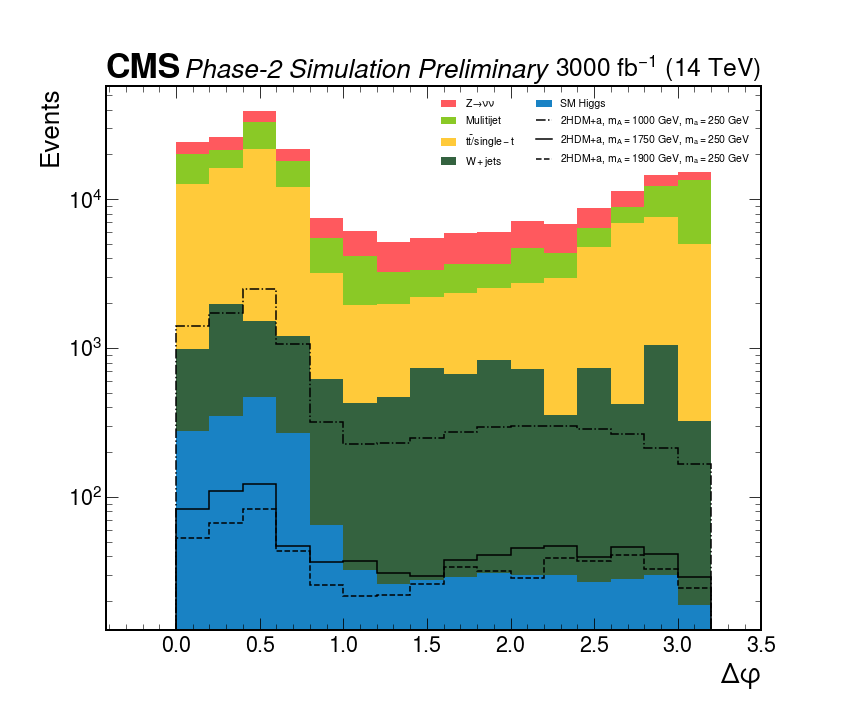
\includegraphics[width=\textwidth]{Chapters/Strategy/selections/AK4_QCD_veto.png}
        \caption{The $\Delta\varphi(\text{any 2 of 4 lead AK4 jets})$ distribution.}
        \label{fig:dphi2o4ak4}
    \end{subfigure}
    \caption{The distributions of the various $\Delta\varphi$ in the backgrounds and the $m_\mathrm{A} =1000$, $1750$, and $\GeV{1900}$, $m_\mathrm{a} = \GeV{250}$ signals with each selection except for any of the $\Delta\varphi$ cuts applied.}
    \label{fig:dphi}
\end{figure}

\begin{sidewaystable}
\centering
\caption{Yields for three chosen signals and the predominant backgrounds.}
\begin{adjustbox}{width=10in}
\begin{tabular}{|c|c|c|c|c|c|c|c|c|}
\hline
 & Z$\to\nu\nu$ & W+jets & Multijet & t$\bar{\mathrm{t}}$/single-t & SM h & $m_\mathrm{A}=\GeV{1000}$, $m_\mathrm{a}=\GeV{250}$ & $m_\mathrm{A}=\GeV{1750}$, $m_\mathrm{a}=\GeV{250}$ & $m_\mathrm{A}=\GeV{1900}$, $m_\mathrm{a}=\GeV{250}$  \\
\hline
Initial                                          & $1226000000\pm40000$ & $214600000000\pm500000$ & $2141000000\pm50000$ & $489500000\pm20000$  & $1929000\pm1000$ & $103100\pm300$ & $188500\pm400$ & $340000\pm600$ \\
$N_\text{leptons} = 0$                           & $1016000000\pm30000$ & $84670000000\pm300000$  & $1457000000\pm40000$ & $101600000\pm10000$  & $701000\pm800$   & $67160\pm260$  & $124500\pm400$ & $224700\pm500$ \\
\ptmiss $> \GeV{300}$                                  & $8339000\pm3000$     & $2595000\pm2000$        & $1103000\pm1000$     & $1288000\pm1000$     & $6647\pm82$      & $28500\pm170$  & $5198\pm72$    & $7374\pm86$    \\
$N_\text{h-tagged AK8} > 0$                      & $114500\pm100$       & $26670\pm80$            & $230800\pm300$       & $226300\pm300$       & $2624\pm35$      & $13140\pm80$   & $1556\pm29$    & $1555\pm28$    \\
min \pt (AK8 jets) $> \GeV{300}$               & $51860\pm90$         & $13380\pm50$            & $126600\pm200$       & $141600\pm200$       & $1811\pm30.$     & $10270\pm70$   & $1066\pm25$    & $983.1\pm22.7$ \\
$N_\text{AK4} > 1$                               & $51860\pm90$         & $13380\pm50$            & $126600\pm200$       & $141600\pm200$       & $1811\pm30$      & $10270\pm70$   & $1066\pm25$    & $983.1\pm22.7$ \\
min $\Delta\varphi$(AK8, \ptmiss) $> 1$          & $47110\pm80$         & $12370\pm50$            & $60630\pm140$        & $97180\pm160$        & $1769\pm30$      & $10050\pm70$   & $847.8\pm21.8$ & $644.5\pm18.0$ \\
$3>\text{min }\Delta\varphi$(AK4, \ptmiss)$>1$   & $29520\pm70$         & $7822\pm39$             & $26900\pm100$        & $27690\pm80$         & $1289\pm25$      & $6891\pm60$    & $505.4\pm17.0$ & $345.8\pm13.8$ \\
$\Delta\varphi(\text{2 AK8 jets}) < 3$           & $29460\pm60$         & $7820\pm39$             & $26850\pm100$        & $27650\pm80$         & $1289\pm25$      & $6882\pm60$    & $504.8\pm17.0$ & $344.9\pm13.8$ \\
$\Delta\varphi(\text{2 of 4 lead AK4 jets}) < 3$ & $28800\pm60$         & $7769\pm39$             & $26640\pm100$        & $27050\pm80$         & $1282\pm25$      & $6795\pm60$    & $496.3\pm16.9$ & $339.8\pm13.7$ \\
min \mt $> \GeV{600}$                          & $27040\pm60$         & $7116\pm37$             & $26180\pm100$        & $26340\pm80$         & $1267\pm25$      & $6618\pm59$    & $483.9\pm16.7$ & $321.4\pm13.3$ \\
\hline
AK8 jet on Higgs mass                            & $5718\pm30$          & $1799\pm20.0$           & $8830\pm60$          & $10360\pm50$         & $884.9\pm21.1$   & $4324\pm48$    & $301.3\pm13.3$ & $188.4\pm10.5$ \\
\hline
\end{tabular}
\end{adjustbox}
\label{tab:cutflow}
\end{sidewaystable}
